\chapter{Introducción}

\section{Elementos pasivos y activos}

Los elementos pasivos que se han estudiado hasta ahora en cursos previos son la resistencia, el condensador y el inductor. Estos elementos son capaces de modificar una señal de entrada y producir una señal de salida, sin necesidad de utilizar fuentes de alimentación externa. Por ejemplo, en el filtro paso bajo, existe una señal de salida y(t) al aplicar una entrada x(t), y el circuito no requiere de una fuente de alimentación independiente para operar. La señal de salida siempre es menor que la señal de entrada, es decir, los elementos pasivos no pueden amplificar la señal de entrada, sólo atenuarla.

Los elementos activos requieren una fuente de alimentación externa para poder producir una salida. La fuente (por ejemplo, $V_{CC}$) es independiente de la señal de entrada x(t), y el circuito consume potencia externa para producir la señal de salida y(t). Estos circuitos son capaces de amplificar señales de entrada, es decir, la señal de salida puede ser mayor que la señal de entrada. Ejemplos de componentes activos son el diodo, el transistor de unión bipolar (BJT) y el transistor de efecto de campo (MOSFET).

En la Figura \ref{elem_pasivos_activos} se muestran los principales elementos pasivos y activos, junto con la forma que tienen las ecuaciones de funcionamiento de cada uno de ellos. Se observa que los elementos pasivos son lineales (la salida es una combinación lineal de la entrada), mientras que los elementos activos son no lineales (la salida es exponencial o cuadrática con respecto a la entrada).

Los elementos activos son utilizados en la industria microelectrónica por su capacidad para procesar información tanto analógica como digital, en amplificadores de audio, sistemas de comunicación por radio y en microprocesadores (de escritorio, portátiles o de teléfonos). 

\begin{figure}[H]
\centering
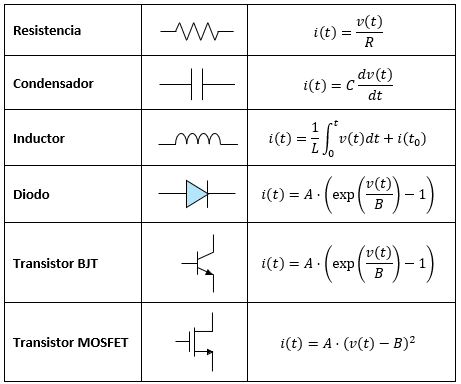
\includegraphics{figuras/elem_pasivos_activos.png}
\caption{Elementos pasivos: resistencia, condensador, inductor, y elementos activos: diodo, transistor BJT, transistor MOSFET, con sus ecuaciones de funcionamiento.}
\label{elem_pasivos_activos}
\end{figure}

\section{La Ley de Moore}

Los circuitos microelectrónicos actuales contienen miles de millones de transistores. Desde la década de 1960 hasta el 2018 se fabricaron más de $13\times{}10^{21}$ transistores \cite{laws2018}. En comparación, la vía láctea tiene entre 100 y 400 mil millones de estrellas ($400\times{}10^9$). Un solo circuito integrado actualmente puede integrar hasta $50\times{}10^9$ transistores individuales en el mismo encapsulado. Esto convierte al transistor en el artefacto producido con más frecuencia por la humanidad en toda su historia.

Los transistores se construyen principalmente con silicio, que se obtiene de la arena, siendo uno de los materiales más abundantes de la corteza terrestre. Con la invención del transistor MOS (metal-óxido-semiconductor), hay quienes dicen que se alcanzó la meta de los alquimistas, que querían transformar un material de bajo costo como la arena, en un material más costoso y de mayor utilidad.

La cantidad de transistores que se integran en procesadores móviles de Apple se cita en la Tabla \ref{tabla_ley_moore}. Para evitar confusiones con la literatura, se destaca que en inglés la palabra ``\textit{billion}''\ equivale a mil millones ($10^9$), que no es lo mismo que un billón en español ($10^{12}$). Por otro lado, en la tabla se indica el año de producción y el proceso de fabricación, que describe la longitud del canal, que es la dimensión más pequeña que puede tener un transistor.

\begin{table}[H]
    \centering
    \caption{Cantidad de transistores en procesadores de Apple.}
    \label{tabla_ley_moore}
    \begin{tabular}{|c|c|c|c|}
        \hline \textbf{Procesador} & \textbf{Año} & \textbf{Cantidad de transistores}  & \textbf{Proceso} \\
         & & \textbf{(en miles de millones)} & (nm) \\
        \hline A7 & 2013 & 1 & 28 \\
        A8 & 2014 & 2 & 20 \\
        A9 & 2015 & 3.3 & 14 \\
        A10 & 2016 & 3.3 & 14 \\
        A11 & 2017 & 4.3 & 10 \\
        A12 & 2018 & 6.9 & 7 \\
        A13 & 2019 & 8.5 & 7 \\
        A14 & 2020 & 11.8 & 5 \\
        A15 & 2021 & 15 & 5 \\
        \hline
    \end{tabular}
\end{table}

La Ley de Moore \cite{moore1965} es una ecuación empírica, propuesta por Gordon Moore en 1965, que dice que la cantidad de transistores dentro de un circuito integrado monolítico se duplica aproximadamente cada dos años. Según la información de la tabla anterior, la tendencia continúa, y se puede apreciar en la gráfica de la Figura 2. Esto sucede con la mayoría de los circuitos integrados de distintas compañías, como por ejemplo Intel, AMD, NVIDIA. 

\begin{figure}[H]
\centering
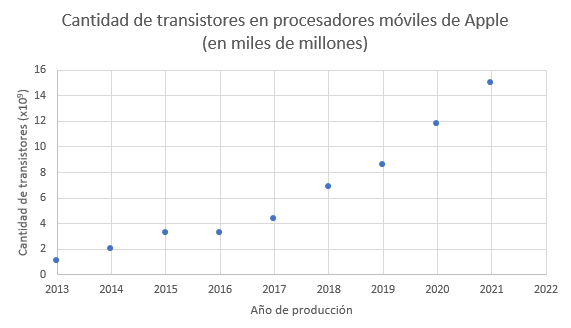
\includegraphics{figuras/ley_moore_apple.png}
\caption{Cantidad de transistores en procesadores de Apple (en miles de millones).}
\label{ley_moore_apple}
\end{figure}

Además, conforme pasa el tiempo los transistores se vuelven cada vez más pequeños. Esto permite colocar cada vez más dispositivos dentro del mismo espacio, y a la vez reducir el consumo de potencia, permitiendo que los circuitos operen más rápido. La teoría de escalamiento de Dennard \cite{dennard1974}, propuesta por Robert Dennard en 1974, establece que es posible reducir las dimensiones de un transistor al escalarlo con un parámetro $\kappa$, si se ajustan los otros parámetros por el mismo factor. Un resumen de los parámetros de escalamiento se muestra en la Tabla \ref{tabla_escalamiento_dennard}. Se observa que las dimensiones de un dispositivo se pueden reducir $\kappa$ veces, si se reduce la tensión y la corriente por ese mismo factor, con lo que la potencia que disipa el transistor escala por $\kappa^2$.

\begin{table}[H]
    \centering
    \caption{Escalamiento de Dennard de acuerdo con un factor $\kappa$ \cite{dennard1974}.}
    \label{tabla_escalamiento_dennard}
    \begin{tabular}{|l|c|}
        \hline \textbf{Parámetro del dispositivo} & \textbf{Factor de escalamiento} \\
        \hline
        Dimensiones del dispositivo $L, W, t_{ox}$ & $1/\kappa$ \\
        Concentración de dopado $N_A, N_D$         & $\kappa$   \\
        Tensión $V$                                & $1/\kappa$ \\
        Corriente $I$                              & $1/\kappa$ \\
        Capacitancia $C = \epsilon A / d$          & $1/\kappa$ \\
        Retardo (delay) $RC = VC/I$                & $1/\kappa$ \\
        Consumo de potencia $P = VI$               & $1/\kappa^2$ \\
        Densidad de potencia $P/A=VI/A$            & $1$ \\
        \hline
    \end{tabular}
\end{table}

Tanto la Ley de Moore como el escalamiento de Dennard se han mantenido vigentes, aunque en la actualidad se están encontrando barreras físicas que impiden continuar con esta tendencia. Uno de los problemas más grandes que existe en la actualidad es la alta densidad de potencia en los circuitos integrados, ya que, si bien es cierto la potencia de cada transistor individual disminuye, se integran cada vez más dispositivos en el mismo tamaño del chip. En la Tabla 2 se observó que la densidad de potencia no escala, sino que se mantiene constante. Esto hace que los circuitos integrados modernos tengan densidades de potencia muy elevadas, lo que se traduce en la generación de calor, que debe ser extraído del circuito por medio de disipadores de calor. Una solución consiste en apagar las partes del circuito integrado que no están en uso, y dividir los procesadores en núcleos de baja potencia o alto rendimiento.

Además, los transistores modernos son dispositivos de escala nanométrica, con una separación entre terminales de apenas 20 \AA\ (la unidad es Angstrom, 1 \AA\ = 0.1 nm). En estos dispositivos, existen efectos cuánticos como por ejemplo el Efecto Túnel, que convierten al dispositivo en un ``cortocircuito'' si no se compensa, por lo que se están buscando alternativas para continuar con las demandas de la industria.
